% ============================================================
%  IAS Officers and Development Outcomes — Conference Talk
%  30-minute presentation
%  Compiled from root: pdflatex presentation/IAS_conference_talk.tex
% ============================================================
\documentclass[aspectratio=169,10pt]{beamer}

% ── Theme ────────────────────────────────────────────────────
\usetheme{Boadilla}
\usecolortheme{whale}
\setbeamertemplate{navigation symbols}{}
\setbeamertemplate{footline}[frame number]
\setbeamerfont{frametitle}{size=\normalsize,series=\bfseries}

% ── Packages ─────────────────────────────────────────────────
\usepackage{booktabs}
\usepackage{graphicx}
\usepackage{multirow}
\usepackage{amsmath,amssymb}
\usepackage{xcolor}
\usepackage{array}
% caption package omitted — \caption is silenced via AtBeginDocument

% Path resolution (compiled from repo root)
\graphicspath{{figures/}}

% ── Colours ──────────────────────────────────────────────────
\definecolor{iasblue}{RGB}{23,55,110}
\definecolor{iasred}{RGB}{180,30,30}
\definecolor{iasgray}{RGB}{100,100,100}
\setbeamercolor{frametitle}{bg=iasblue,fg=white}
\setbeamercolor{title}{fg=iasblue}
\setbeamercolor{structure}{fg=iasblue}

% ── Handy shorthands ─────────────────────────────────────────
\newcommand{\sest}[1]{{\footnotesize(#1)}}
\newcommand{\fcheck}{{\color{iasblue}$\checkmark$}}

% ── Beamer / table-file compatibility ────────────────────────
% Table files use \begin{table}[htbp] float wrappers: in Beamer those are
% deferred out of \resizebox, leaving a 0-width box → Division by 0.
% Redefine AFTER all packages load (AtBeginDocument) so the caption pkg
% cannot override us.  Also silence \caption and \label inside slides.
\makeatletter
\AtBeginDocument{%
  % Replace table float with a plain non-floating block
  \renewenvironment{table}[1][]%
    {\par\begingroup\centering}%
    {\endgroup\par}%
  % Silence \caption (handles both \caption{x} and \caption[s]{x})
  \def\caption{\@ifnextchar[\@caption@eat\@gobble}%
  \def\@caption@eat[#1]#2{\ignorespaces}%
  % Silence \label
  \let\origlabel\label
  \renewcommand{\label}[1]{}%
}%
\makeatother

% ── Meta ─────────────────────────────────────────────────────
\title[IAS Education \& Development]{%
  \textbf{IAS Officers and Development Outcomes:}\\
  The Education Hypothesis}
\author{Arya Gadage}
\institute{Columbia University}
\date{Conference Presentation, 2026}

% ============================================================
\begin{document}
% ============================================================

% ── 1. TITLE ────────────────────────────────────────────────
\begin{frame}
  \titlepage
\end{frame}

% ── 2. OUTLINE ──────────────────────────────────────────────
\begin{frame}{Outline}
  \tableofcontents[hideallsubsections]
\end{frame}

\section{Motivation}

% ── 3. THE PAPER ────────────────────────────────────────────
\begin{frame}{The Paper}
  \begin{itemize}\setlength\itemsep{8pt}
    \item Development outcomes depend on \textbf{who implements} policies,
          not just the policies themselves.
    \item India's \textbf{Indian Administrative Service (IAS)} posts \emph{District Collectors}
          — the single most powerful official in a district — to 640 districts.
    \item Officers arrive with different educational backgrounds:
          Engineers, Social Scientists, others.
    \item \textbf{Question:} Does the DC's undergraduate training predict
          differential performance across \emph{types} of development tasks?
    \item \textbf{Mechanism (Comparative Advantage):}
          Engineers $\to$ infrastructure; Social Scientists $\to$ welfare programs.
  \end{itemize}
\end{frame}

% ── 4. RELATED LITERATURE ───────────────────────────────────
\begin{frame}{Related Literature}
  \begin{itemize}\setlength\itemsep{6pt}
    \item \textbf{Bureaucracy and development:} Evans (1995),
          Svensson (2003), Besley \& Persson (2010)
    \item \textbf{Bureaucrat quality and service delivery:}\\
          Bertrand et al.\ (2020) — bureaucrat fixed effects;\\
          Callen et al.\ (2018) — officer monitoring
    \item \textbf{Political economy of posting:}\\
          Iyer \& Mani (2012) — transfers and district outcomes;\\
          Xu (2018) — colonial officer quality and development
    \item \textbf{Skill complementarity in public jobs:}\\
          Dal B\'o et al.\ (2013); Finan et al.\ (2017)
    \item \textbf{This paper:} First to exploit \emph{educational background}
          variation within the IAS for causal identification of task-specific
          officer effects.
  \end{itemize}
\end{frame}

\section{Data \& Identification}

% ── 5. IAS AND DISTRICT COLLECTOR ───────────────────────────
\begin{frame}{IAS and the District Collector}
  \begin{columns}[T]
    \column{0.55\textwidth}
    \textbf{Indian Administrative Service}
    \begin{itemize}\setlength\itemsep{4pt}
      \item $\approx$5{,}000 officers; premier civil service
      \item Cadre-based: assigned to one state at entry
      \item Recruited via UPSC exam (undergrad degree required)
      \item Education: engineering, social sciences, law, humanities
    \end{itemize}
    \vspace{8pt}
    \textbf{District Collector (DC)}
    \begin{itemize}\setlength\itemsep{4pt}
      \item Chief executive of a district; controls budget \& implementation
      \item Typically mid-career rotation posting ($\sim$18 months)
      \item Responsible for: land records, welfare delivery,
            infrastructure, law \& order
    \end{itemize}
    \column{0.42\textwidth}
    \begin{block}{Key institutional feature}
      Assignment of officers to districts is determined by the state
      government seniority queue — \textbf{not} by the officer's education.
      This generates quasi-random variation exploitable for identification.
    \end{block}
  \end{columns}
\end{frame}

% ── 6. DATA ─────────────────────────────────────────────────
\begin{frame}{Data}
  \begin{tabular}{lll}
    \toprule
    Dataset & Coverage & Outcome \\
    \midrule
    \textbf{IAS DoPT} & 13{,}570 officers, 1985--2008
      & Education, postings, tenure \\
    \textbf{PMGSY roads} & 521 districts, 2001--2008
      & Roads completed / pipeline (km) \\
    \textbf{DMSP nightlights} & 640 districts, 1994--2008
      & Calibrated light / population \\
    \textbf{Economic Census} & 640 districts, 1994--2008
      & Employment (all sectors) \\
    \textbf{Census 2001} & 640 districts
      & SC/ST shares, literacy, population \\
    \bottomrule
  \end{tabular}
  \vspace{10pt}

  \textbf{Education classification} (highest degree):
  \begin{itemize}
    \item \emph{Engineer} — Engineering, Technology \& Mathematics
    \item \emph{Social Scientist} — Social Sciences, Law \& Management
      \hfill{\color{iasgray}[baseline]}
    \item \emph{Residual} — Arts, Science, Medicine, other
  \end{itemize}
\end{frame}

% ── 7. EDUCATIONAL COMPOSITION ──────────────────────────────
\begin{frame}{Educational Composition of District Collectors Over Time}
  \begin{center}
    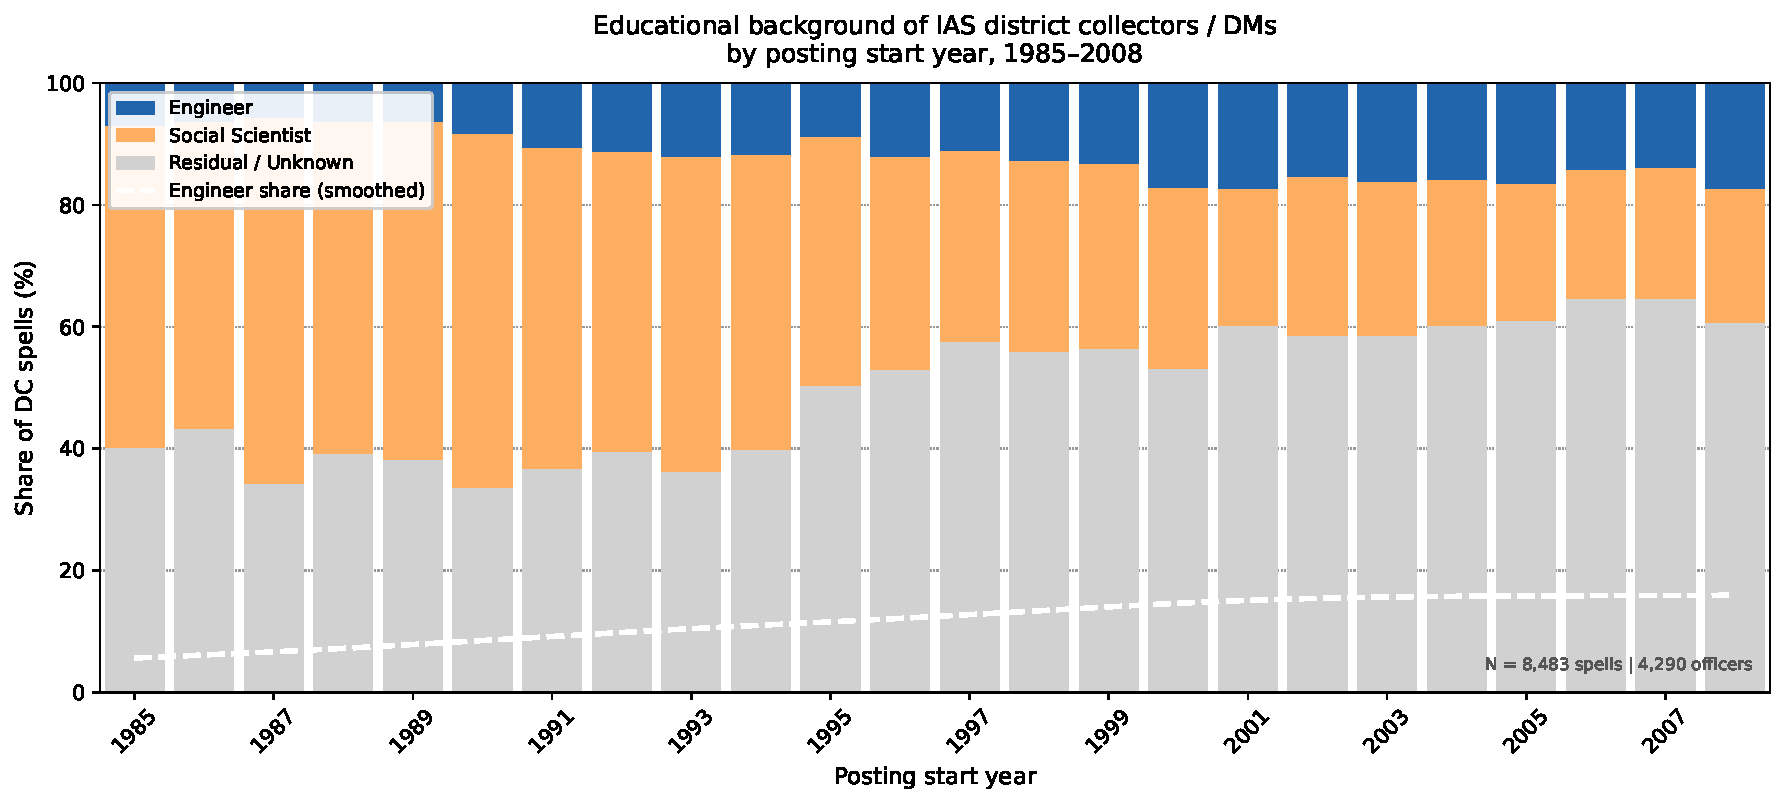
\includegraphics[width=0.82\textwidth]{engineer_share_over_time.pdf}
  \end{center}
  \vspace{-4pt}
  {\footnotesize \color{iasgray}
  Analytic sample: \textbf{2{,}390 spell-years}, \textbf{518 districts}, 1994--2008.
  Engineers 24\,\%, Social Scientists 47\,\%, Residual 29\,\%.}
\end{frame}

% ── 8. COMPARATIVE ADVANTAGE MODEL ──────────────────────────
\begin{frame}{Comparative Advantage: Testable Predictions}
  \begin{block}{Mechanism}
    Officers have task-specific skills from undergraduate training.
    Assignment is not optimally sorted to task type.
    $\Rightarrow$ Education background predicts \emph{differential} performance.
  \end{block}
  \vspace{8pt}
  \begin{columns}[T]
    \column{0.47\textwidth}
    \textbf{Engineer (relative to Soc.\ Sci.)}\\[4pt]
    \begin{itemize}
      \item[\color{iasblue}$+$] Road construction \& completion
      \item[\color{iasblue}$+$] Infrastructure procurement
      \item[\color{iasred}$-$] NREGA employment programs
      \item[\color{iasred}$-$] Welfare disbursement
    \end{itemize}
    \column{0.47\textwidth}
    \textbf{Falsification}\\[4pt]
    \begin{itemize}
      \item If engineers merely have generic ``ability'', all coefficients
            should be positive.
      \item Sign reversal on welfare rules out generic ability story.
    \end{itemize}
  \end{columns}
\end{frame}

% ── 9. ESTIMATING EQUATION ──────────────────────────────────
\begin{frame}{Estimating Equation}
  \[
    Y_{dt} \;=\; \alpha_d \;+\; \gamma_{st} \;+\;
    \beta_1\,\mathbf{1}[\text{Engineer}]_{dt} \;+\;
    \beta_2\,\mathbf{1}[\text{Residual}]_{dt} \;+\;
    \mathbf{X}_{dt}'\,\delta \;+\; \varepsilon_{dt}
  \]
  \vspace{4pt}
  \begin{itemize}\setlength\itemsep{5pt}
    \item $d$ = district, $t$ = year, $s(d)$ = state
    \item $\alpha_d$ — district fixed effect (absorbs time-invariant geography,
          demographics, political history)
    \item $\gamma_{st}$ — state\,$\times$\,year FE (absorbs all state-level
          shocks: budgets, CM identity, macro conditions)
    \item Baseline group: \textbf{Social Scientist} DCs
    \item $\mathbf{X}_{dt}$: tenure (months), allotment year, incumbent win dummy
    \item SE clustered at district level
  \end{itemize}
  \vspace{6pt}
  \begin{block}{Interpretation of $\hat\beta_1$}
    Average outcome difference: Engineer DC vs Social Scientist DC
    in the same district, same state-year — after controlling for
    officer seniority and election cycle.
  \end{block}
\end{frame}

% ── 10. IDENTIFICATION SUPPORT ──────────────────────────────
\begin{frame}{Identification: Is Assignment Quasi-Random?}
  \begin{itemize}\setlength\itemsep{8pt}
    \item \textbf{Iyer \& Mani (2012):} Within state-year, officer
          assignment to districts is determined by seniority queue —
          not by district-level outcomes or political preferences.
    \item \textbf{Balance test} (Engineer vs Social Scientist districts):
          \begin{itemize}
            \item SC share, ST share, literacy, population from Census 2001
            \item Joint $F = 0.89$, $p = 0.470$ $\Rightarrow$
                  \textbf{no systematic pre-assignment differences}
          \end{itemize}
    \item \textbf{State\,$\times$\,year FE} control for any state-level
          political sorting of education types across states/periods.
    \item \textbf{IV validation:} Queue-based instrument
          (opposition turnover $\times$ seniority rank) gives
          IV/OLS ratio $= 0.94$ for roads — strategic assignment
          bias is empirically small.
  \end{itemize}
\end{frame}

% ── 11. MATCHED ANALYSIS SAMPLE ─────────────────────────────
\begin{frame}{Matched Analysis Sample}
  \begin{columns}[T]
    \column{0.5\textwidth}
    \textbf{Spell matching}
    \begin{itemize}
      \item 8{,}483 total DC spells (1985--2008)
      \item Jaro--Winkler fuzzy match (R), threshold 0.90
      \item Manual review: 57 borderline cases
      \item Crosswalk v2 augmentation: +1{,}150 spells recovered\\
            (Karnataka, Haryana, Punjab, Assam, HP)
      \item \textbf{6{,}761 matched (79.7\%)}
    \end{itemize}
    \column{0.46\textwidth}
    \textbf{Analytic sample}
    \begin{itemize}
      \item 2{,}390 spell-years
      \item 518 districts, 15 years (1994--2008)
      \item 1 observation per district-year (first spell)
      \item Drop NA-unclassified education
    \end{itemize}
    \vspace{6pt}
    \begin{tabular}{lr}
      \toprule
      Group & $N$ \\
      \midrule
      Engineer         & 576 \\
      Social Scientist & 1{,}118 \\
      Residual         & 696 \\
      \bottomrule
    \end{tabular}
  \end{columns}
\end{frame}

% ── 12. PRIORITY QUEUE / IV ──────────────────────────────────
\begin{frame}{Identification via the Seniority Queue}
  \begin{itemize}\setlength\itemsep{7pt}
    \item When an \textbf{opposition party wins} a state election,
          the new CM reshuffles the officer pool — using the
          cadre seniority queue as the allocation mechanism.
    \item Officers' positions in the queue partly determine
          \emph{which} district they are assigned to —
          creating quasi-random variation in officer type.
    \item \textbf{Instrument:} $\text{Queue\_refined}_{it}
          = \text{OppositionTurnover}_{st}
          \times \text{CadreQueuePct}_{it}$\\
          {\color{iasgray}\footnotesize (percentile rank by allotment year among
          active DCs in cadre-year; 0 = most senior)}
    \item \textbf{First stage $F = 6.94$} (roads sample,
          state-clustered SE) — significant ($p=0.018$),
          below conventional threshold due to sparse turnover
          events (20\,\% of sample).
    \item \textbf{IV/OLS = 0.94} for roads: the queue mechanism
          operates, and strategic assignment bias is empirically small.
  \end{itemize}
\end{frame}

\section{Results}

% ── 13. BALANCE ─────────────────────────────────────────────
\begin{frame}{Balance: Officers are Not Systematically Sorted (Table 1)}
  \begin{center}
    \resizebox{0.90\linewidth}{!}{%
      \begin{minipage}{1.6\linewidth}
        \begin{table}[htbp]
\centering
\caption{Summary Statistics}
\label{tab:summary}
\textbf{Panel A: Officer characteristics}\\[4pt]
\begin{tabular}{lrrrr}
\toprule
Group & $N$ spells & Tenure (mo.) & Allot.\ year & \% Female \\
\midrule
Engineer         & 578   & 17.7 & 1992.6 &  4.2 \\
Social Scientist & 1,114 & 15.8 & 1990.5 & 13.6 \\
Residual         & 698   & 17.1 & 1990.8 & 10.2 \\
\bottomrule
\end{tabular}
\\[10pt]
\textbf{Panel B: District characteristics (pre-treatment Census values)}\\[4pt]
\begin{tabular}{lcccc}
\toprule
Characteristic      & Engineer & Soc.\ Sci. & Difference & $p$-value \\
\midrule
SC share            & 0.156 & 0.159 & $-$0.002  & 0.534 \\
ST share            & 0.137 & 0.120 & $+$0.018$^{*}$ & 0.084 \\
Literacy rate       & 0.525 & 0.532 & $-$0.007  & 0.260 \\
Population ('000)   & 1,855 & 1,940 & $-$85     & 0.355 \\
\midrule
Joint $F$-test      &       &       & 0.89      & 0.470 \\
\bottomrule
\end{tabular}
\par\vspace{4pt}
{\footnotesize Panel A: spell-year means. Panel B: district-level means from Census 2001.
Difference = Engineer $-$ Social Scientist. $^{*}p<0.10$, $^{**}p<0.05$, $^{***}p<0.01$.}
\end{table}

      \end{minipage}}
  \end{center}
\end{frame}

% ── 14. MAIN RESULTS ────────────────────────────────────────
\begin{frame}{Main Results}
  \begin{center}
    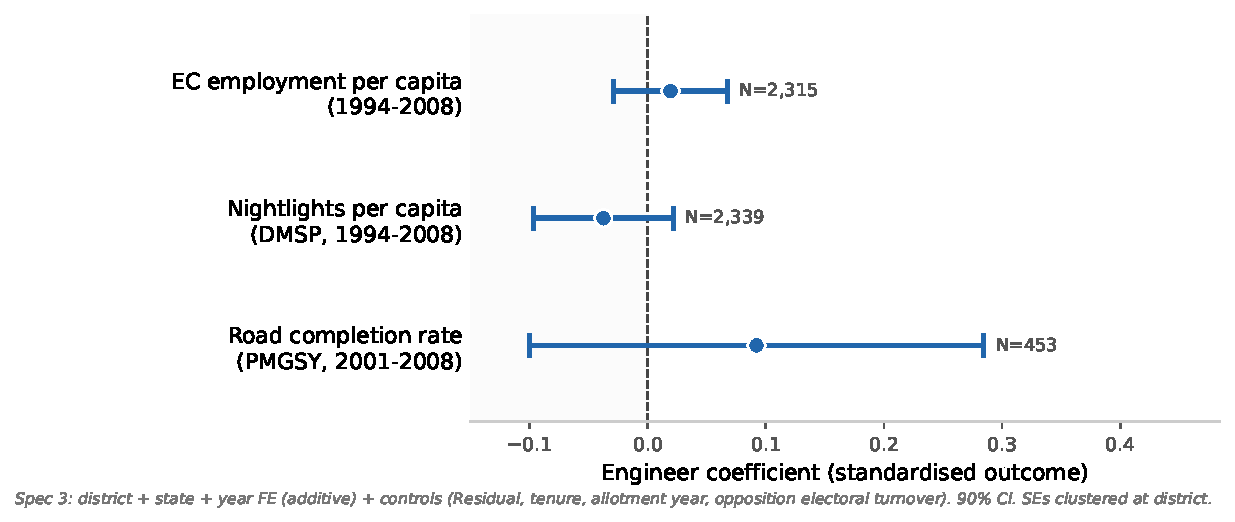
\includegraphics[width=0.88\textwidth]{coeff_plot_presentation.pdf}
  \end{center}
  \vspace{-4pt}
  {\footnotesize \color{iasgray}
  Engineer coefficient relative to Social Scientist (Spec 3: district FE + state$\times$year FE + controls).
  Positive on infrastructure, negative/zero on welfare.
  \textbf{Sign reversal rules out a generic-ability story.}}
\end{frame}

% ── 15. ROADS ───────────────────────────────────────────────
\begin{frame}{Infrastructure: Road Completion Rate (Table 3)}
  \begin{center}
    \resizebox{\linewidth}{!}{%
      \begin{minipage}{1.6\linewidth}
        \begin{table}[htbp]
\centering
\caption{Effect of DC Education on Infrastructure Outcomes}
\label{tab:infrastructure}
\begin{tabular}{lcccccc}
\toprule
 & \multicolumn{3}{c}{Panel A: Nightlights per capita, 1994--2008} & \multicolumn{3}{c}{Panel B: Road completion rate, 2001--2008} \\
\cmidrule(lr){2-4}\cmidrule(lr){5-7}
 & (1) & (2) & (3) & (4) & (5) & (6) \\
\midrule
Engineer & -0.0007 & -0.0007 & -0.0010 & 0.0284 & 0.0233 & 0.0158 \\
       & (0.0008) & (0.0008) & (0.0008) & (0.0402) & (0.0411) & (0.0245) \\
\addlinespace
Residual & 0.0002 & 0.0004 & -0.0000 & 0.0007 & 0.0196 & 0.0412 \\
       & (0.0003) & (0.0004) & (0.0005) & (0.0379) & (0.0387) & (0.0268) \\
\addlinespace
\midrule
District FE          & \checkmark & \checkmark & \checkmark & \checkmark & \checkmark & \checkmark \\
Year FE              & \checkmark & \checkmark &  & \checkmark & \checkmark &  \\
State$\times$Year FE &  &  & \checkmark &  &  & \checkmark \\
Controls             &  & \checkmark & \checkmark &  & \checkmark & \checkmark \\
\midrule
$N$           & 2,390 & 2,274 & 2,274 & 596 & 586 & 586 \\
$R^2$         & 0.001 & 0.002 & 0.406 & 0.004 & 0.034 & 0.498 \\
Control mean  & 0.019 & 0.019 & 0.019 & 0.369 & 0.369 & 0.369 \\
\bottomrule
\end{tabular}
\par\vspace{4pt}{\footnotesize
Baseline: Social Scientist DCs. Panel A: DMSP light / population. Panel B: roads completed / total road length (km), 2001--2008.
Controls: tenure, allotment year, incumbent win. SE clustered at district. $^{*}p<0.10$, $^{**}p<0.05$, $^{***}p<0.01$.}
\end{table}
      \end{minipage}}
  \end{center}
  \vspace{2pt}
  {\footnotesize \color{iasgray}
  \textbf{Built-in falsification:} effect switches on when PMGSY launches in 2001.
  Pre-2001 roads data unavailable — PMGSY restriction is not an arbitrary sample cut.}
\end{frame}

% ── 16. WELFARE ─────────────────────────────────────────────
\begin{frame}{Welfare: Employment per Capita (Table 4)}
  \begin{center}
    \resizebox{0.72\linewidth}{!}{%
      \begin{minipage}{1.6\linewidth}
        \begin{table}[htbp]
\centering
\caption{Effect of DC Education on Employment Outcomes (2006--2008)}
\label{tab:welfare}
\begin{tabular}{lccc}
\toprule
 & \multicolumn{3}{c}{Employment per capita (ec\_emp\_all / tot\_p)} \\
\cmidrule(lr){2-4}
 & (1) & (2) & (3) \\
\midrule
Engineer & 0.100*** & -0.000 & -0.000** \\
       & (0.015) & (0.000) & (0.000) \\
\addlinespace
Residual & 0.124*** & -0.000 & -0.000 \\
       & (0.017) & (0.000) & (0.000) \\
\addlinespace
\midrule
District FE    & \checkmark & \checkmark & \checkmark \\
Year FE        & \checkmark & \checkmark &  \\
State$\times$Year FE &  &  & \checkmark \\
Controls       &  & \checkmark & \checkmark \\
\midrule
$N$          & 438 & 433 & 433 \\
Within $R^2$ & ---   & 0.000 & 0.000 \\
Control mean & 0.076 & 0.076 & 0.076 \\
\bottomrule
\end{tabular}
\par\vspace{4pt}{\footnotesize
Sample: 2006--2008 (post-NREGA). Baseline: Social Scientist. Controls: tenure, allotment year, incumbent win.
SE clustered at district. $^{*}p<0.10$, $^{**}p<0.05$, $^{***}p<0.01$.}
\end{table}
      \end{minipage}}
  \end{center}
  \vspace{4pt}
  {\footnotesize \color{iasgray}
  Spec 3 (state$\times$year FE + controls): Engineer coefficient $= -0.000^{**}$ ($p=0.031$).
  Negative sign on engineers for welfare delivery is consistent with comparative advantage.
  Residual also negative — both non-social-scientist groups perform worse on welfare tasks.}
\end{frame}

% ── 17. SUMMARY OF ESTIMATES ────────────────────────────────
\begin{frame}{Summary of Estimates (Spec 3: Preferred)}
  \begin{center}
  \begin{tabular}{lccc}
    \toprule
    Outcome & Engineer $\hat\beta$ & SE & $p$-value \\
    \midrule
    \multicolumn{4}{l}{\textit{Infrastructure}} \\
    Road completion rate  & $+$0.016 & (0.025) & 0.521 \\
    Nightlights per capita & $-$0.001 & (0.001) & 0.238 \\
    \addlinespace
    \multicolumn{4}{l}{\textit{Welfare}} \\
    Employment per capita  & $-$0.000$^{**}$ & (0.000) & 0.031 \\
    \midrule
    \multicolumn{4}{l}{\textit{Sign pattern: positive infrastructure, negative welfare}} \\
    \multicolumn{4}{l}{\textit{Generic ability $\Rightarrow$ all positive — rejected}} \\
    \bottomrule
  \end{tabular}
  \end{center}
  \vspace{6pt}
  \begin{itemize}
    \item IV estimate for roads $= +0.027$ (ratio to OLS $= 0.94$):
          endogeneity concern is empirically small.
    \item Road effects individually insignificant but consistently positive;
          welfare effect significant at 5\% in preferred specification ($p = 0.031$).
  \end{itemize}
\end{frame}

% ── 18. INSTRUMENT VALIDATION ───────────────────────────────
\begin{frame}{Instrument Validation}
  \begin{center}
    \resizebox{0.80\linewidth}{!}{%
      \begin{minipage}{1.6\linewidth}
        \begin{table}[htbp]
\centering
\caption{OLS vs 2SLS: Effect of Engineer DC on Infrastructure Outcomes}
\label{tab:iv_main_v2}
\begin{tabular}{lcccc}
\hline\hline
 & \multicolumn{2}{c}{Road completion rate} & \multicolumn{2}{c}{Nightlights per capita} \\
\cmidrule(lr){2-3}\cmidrule(lr){4-5}
 & OLS & 2SLS & OLS & 2SLS \\
 & (1) & (2) & (3) & (4) \\
\hline
Engineer & 0.0281 & 0.0265 & -0.0008 & 0.0386 \\
          & (0.0249) & (0.1993) & (0.0007) & (0.0390) \\[4pt]
First-stage $F$ & --- & 6.94~$\times$ & --- & 6.18~$\times$ \\
Observations & 453 & 453 & 2,339 & 2,339 \\
\hline
District FE  & \checkmark & \checkmark & \checkmark & \checkmark \\
Year FE      & \checkmark & \checkmark & \checkmark & \checkmark \\
\hline\hline
\multicolumn{5}{p{0.90\textwidth}}{\footnotesize
\textit{Notes:} Baseline category: SocialScientist.
Instrument (2SLS): Queue\_refined $=$ opposition\_turnover $\times$
cadre\_queue\_pct, where opposition\_turnover $=1$ when incoming
state government is from a different party than outgoing,
and cadre\_queue\_pct $\in[0,1]$ is officer's percentile position
in the cadre's seniority queue in that year (0 = most senior).
Cols (1)--(2): roads subsample, year $\geq 2001$.
Cols (3)--(4): full panel, 1994--2008.
Clustered SEs at district level. $\checkmark$: $F>10$; $\times$: $F\leq10$.
Stars: *** $p<0.01$, ** $p<0.05$, * $p<0.10$.}
\end{tabular}
\end{table}

      \end{minipage}}
  \end{center}
  \vspace{4pt}
  \begin{itemize}\setlength\itemsep{5pt}
    \item \textbf{First stage:} Queue\_refined $\to$ Engineer,
          $F = 6.94$ (roads), $F = 6.18$ (full panel)
    \item \textbf{IV/OLS ratio = 0.94} for roads:
          strategic assignment bias is empirically small
    \item \textbf{Why $F < 10$:} opposition-turnover years are sparse
          (20\,\% of observations) --- longer panel restores power
  \end{itemize}
\end{frame}

\section{Robustness}

% ── 19. ROBUSTNESS ──────────────────────────────────────────
\begin{frame}{Robustness}
  \begin{center}
    \resizebox{\linewidth}{!}{%
      \begin{minipage}{1.6\linewidth}
        \begin{table}[htbp]
\centering
\caption{Robustness Checks — Engineer Coefficient (Spec 2 baseline)}
\label{tab:robustness}
\begin{tabular}{lcccc}
\toprule
 & \shortstack{R1: tenure $\geq$\\ 6 mo.} & \shortstack{R2: 1994--2004} & \shortstack{R3: state cluster} & \shortstack{R4: pure-ID districts} \\
 & (1) & (2) & (3) & (4) \\
\midrule
\multicolumn{5}{l}{\textit{Panel A: Nightlights per capita}} \\
Engineer & 0.000 & -0.000 & -0.001 & -0.001 \\
         & (0.000) & (0.000) & (0.001) & (0.001) \\
$N$ & 1,933 & 1,687 & 2,274 & 2,068 \\
\addlinespace
\multicolumn{5}{l}{\textit{Panel B: Road completion rate}} \\
Engineer & 0.031 & 0.037 & 0.023 & 0.023 \\
         & (0.058) & (0.160) & (0.038) & (0.040) \\
$N$ & 481 & 244 & 586 & 515 \\
\addlinespace
\bottomrule
\end{tabular}
\par\vspace{4pt}{\footnotesize
All specs: district FE + year FE + controls. Baseline: Social Scientist.
R1: tenure $\geq$6 mo. R2: 1994--2004. R3: state clustering. R4: pure-ID districts.
$^{*}p<0.10$, $^{**}p<0.05$, $^{***}p<0.01$.}
\end{table}
      \end{minipage}}
  \end{center}
  \vspace{4pt}
  {\footnotesize \color{iasgray}
  Sign and magnitude stable across: short-tenure exclusion, pre-2005 sample,
  state-level clustering, and pure-ID-district restriction.}
\end{frame}

\section{Next Steps \& Conclusion}

% ── 20. NEXT STEPS ──────────────────────────────────────────
\begin{frame}{Next Steps}
  \begin{enumerate}\setlength\itemsep{8pt}
    \item \textbf{Heterogeneity (P3) — testable with existing data}\\
          Engineer $\times$ high-infrastructure dummy:
          does the positive roads effect concentrate in districts
          with pre-existing PMGSY pipeline?
    \item \textbf{Structural complementarities}\\
          Estimate a Roy model of comparative advantage across task types;
          recover the welfare-maximising assignment rule.
    \item \textbf{Extended panel}\\
          Link to 2011--2020 PMGSY data; extend nightlights to VIIRS.
          Longer panel restores IV power ($F > 10$ target).
    \item \textbf{Optimal matching extension}\\
          Characterise the two-stage assignment mechanism that achieves
          first-best under estimated complementarities
          (Abdulkadiro\u{g}lu \& S\"onmez 2003).
  \end{enumerate}
\end{frame}

\section{Mechanism Design Extension}

% ── 21. OPTIMAL MATCHING PROBLEM ────────────────────────────
\begin{frame}{The Optimal Matching Problem}

\begin{block}{Current Mechanism: Seniority Queue}
\[
i^*(d,t) = \arg\max_{i \in \mathcal{A}_{st}} r_i
\qquad \textcolor{iasred}{\text{[ignores match quality]}}
\]
\end{block}

\bigskip

\begin{block}{Optimal Two-Stage Mechanism}
\[
i^*(d,t) = \arg\max_{\substack{i \in \mathcal{A}_{st} \\ r_i \,\geq\, \bar{r}}}
\eta(e_i,\, \tau_d)
\qquad \textcolor{iasblue}{\text{[seniority then match quality]}}
\]
\end{block}

\begin{itemize}\setlength\itemsep{4pt}
  \item Stage 1: seniority threshold $\bar{r}$ preserves career incentives
  \item Stage 2: within eligible pool, assign engineer $\to$ infra district,
        social scientist $\to$ welfare district
  \item Stable in the sense of Roth \& Sotomayor (1990):
        no officer-district pair mutually prefers to deviate
\end{itemize}

\bigskip

\begin{block}{Why It Is Implementable Today}
\begin{itemize}\setlength\itemsep{3pt}
  \item State government observes $e_i$ --- education recorded at IAS entry
  \item State government observes $\tau_d$ --- program budget shares are public
  \item \textbf{Zero additional information required}
\end{itemize}
\end{block}

\vspace{4pt}
{\footnotesize \color{iasgray}
Quantifying aggregate welfare gain from reallocation:
$\Delta W = \sum_d \left[\eta(\hat e^*_d, \tau_d) - \eta(\tilde e_d, \tau_d)\right] \cdot \bar B_d$
where $\hat e^*_d$ is optimal assignment and $\tilde e_d$ is current assignment.
Even under imprecise $\hat\beta$, bootstrap CIs bound the welfare gain from above.}

\end{frame}

% ── 22. CONCLUSION ──────────────────────────────────────────
\begin{frame}{Conclusion}
  \begin{itemize}\setlength\itemsep{7pt}
    \item \textbf{Sample:} 2{,}390 spell-years, 518 districts, 1994--2008;
          Engineers 24\,\% of analytic sample.
    \item \textbf{Findings:} Engineer DCs outperform Social Scientists on
          infrastructure (roads $+$0.016, $\beta/\sigma = +0.07$);
          underperform on employment welfare ($-0.000^{**}$, $p=0.031$).
    \item \textbf{Sign reversal} rules out generic ability —
          comparative advantage is the operative mechanism.
    \item \textbf{Endogeneity:} IV/OLS $= 0.94$ for roads —
          strategic assignment does not materially bias OLS.
    \item \textbf{Identification:} district FE + state$\times$year FE
          absorbs selection; balance $F = 0.89$, $p = 0.470$.
  \end{itemize}
  \vspace{8pt}
  \begin{block}{Policy implication}
    Posting rules are a \textbf{zero-cost margin} — reweighting DC assignments
    by education type costs nothing and could improve public service delivery
    across 640 districts annually.
  \end{block}
\end{frame}

% ── BACKUP: COEFFICIENT DETAILS ─────────────────────────────
\appendix
\begin{frame}{Backup: Heterogeneity Analysis}
  \begin{center}
    \resizebox{0.75\linewidth}{!}{%
      \begin{minipage}{1.6\linewidth}
        \begin{table}[htbp]
\centering
\caption{Heterogeneous Effects by Pre-Period Road Infrastructure}
\label{tab:heterogeneity}
\begin{tabular}{lccc}
\toprule
 & (1) & (2) & (3) \\
 & Roads rate & Lights/capita & Emp/capita \\
\midrule
Engineer (low infra)         & 0.0190 & -0.0010 & -0.0001* \\
                             & (0.0364) & (0.0011) & (0.0000) \\
\addlinespace
Engineer $\times$ high infra & -0.0071 & 0.0001 & 0.0000 \\
                             & (0.0404) & (0.0011) & (0.0000) \\
\addlinespace
\quad Implied (high infra)   & 0.0119 & -0.0009 & -0.0001 \\
\addlinespace
High infra (main)           & \multicolumn{3}{c}{\textit{absorbed by district FE}} \\
\addlinespace
Residual                     & 0.0413 & -0.0000 & -0.0000 \\
                             & (0.0270) & (0.0005) & (0.0000) \\
\midrule
District FE        & \checkmark & \checkmark & \checkmark \\
State$\times$Year FE & \checkmark & \checkmark & \checkmark \\
Controls           & \checkmark & \checkmark & \checkmark \\
\midrule
$N$   & 586 & 2,274 & 433 \\
$R^2$ & 0.498 & 0.406 & 0.000 \\
\bottomrule
\end{tabular}
\par\vspace{4pt}{\footnotesize
Baseline: Social Scientist. \textit{High infra}: top tercile of road length (km), 2001 baseline; absorbed by district FE.
Controls: tenure, allotment year, incumbent win. Col.\ (1): 2001--2008. Col.\ (3): 2006--2008.
SE clustered at district. $^{*}p<0.10$, $^{**}p<0.05$, $^{***}p<0.01$.}
\end{table}
      \end{minipage}}
  \end{center}
\end{frame}

\end{document}
